\documentclass[11pt,oneside,openany]{book}

\usepackage[a4paper,margin=1in,headheight=14pt]{geometry}
\usepackage[T1]{fontenc}
\usepackage{lmodern}
\usepackage{microtype}
\usepackage{parskip}
\usepackage{amsmath,amssymb,mathtools}
\usepackage{booktabs,array,longtable}
\usepackage{enumitem}
\usepackage{graphicx}
\usepackage{xcolor}
\usepackage{tikz}
\usepackage{pgfplots}
\pgfplotsset{compat=1.18}
\usepackage{tcolorbox}
\usepackage{titlesec}
\usepackage{fancyhdr}
\usepackage{listings}
\usepackage{caption}
\usepackage{hyperref}
\usepackage{xurl}
\usepackage{imakeidx}

\definecolor{econnavy}{HTML}{123B4A}
\definecolor{econred}{HTML}{C6535E}
\definecolor{econink}{HTML}{20252A}
\definecolor{econmuted}{HTML}{5C6870}
\definecolor{econpale}{HTML}{EDF3F5}
\definecolor{econfog}{HTML}{F7F8F7}

\hypersetup{
  colorlinks=true,
  linkcolor=econnavy,
  citecolor=econnavy,
  urlcolor=econred,
  pdftitle={Economics: Choices, Institutions, Power, and Prosperity},
  pdfauthor={Scott Brodie Forsyth}
}

\setlength{\parindent}{0pt}
\setlength{\parskip}{6pt}
\setlist{itemsep=2pt,topsep=3pt}
\setcounter{secnumdepth}{2}
\setcounter{tocdepth}{1}

\titleformat{\chapter}[display]
  {\normalfont\sffamily\bfseries\color{econnavy}\raggedright}
  {\fontsize{12}{14}\selectfont\chaptertitlename\ \thechapter}
  {8pt}{\fontsize{24}{28}\selectfont}
\titleformat{\section}
  {\normalfont\sffamily\bfseries\color{econnavy}}{\thesection}{0.6em}{}
\titleformat{\subsection}
  {\normalfont\sffamily\bfseries\color{econred}}{\thesubsection}{0.6em}{}
\titlespacing*{\chapter}{0pt}{0pt}{24pt}
\titlespacing*{\section}{0pt}{18pt}{6pt}
\titlespacing*{\subsection}{0pt}{12pt}{4pt}

\pagestyle{fancy}
\fancyhf{}
\fancyhead[L]{\sffamily\small\color{econmuted}ECONOMICS}
\fancyhead[R]{\sffamily\small\color{econmuted}\nouppercase{\leftmark}}
\fancyfoot[C]{\sffamily\small\thepage}
\renewcommand{\headrulewidth}{0pt}

\newtcolorbox{keybox}[1][]{
  colback=econpale,colframe=econnavy,boxrule=0.6pt,
  arc=2pt,left=8pt,right=8pt,top=7pt,bottom=7pt,#1}
\newtcolorbox{warningbox}[1][]{
  colback=red!4,colframe=econred,boxrule=0.6pt,
  arc=2pt,left=8pt,right=8pt,top=7pt,bottom=7pt,#1}
\newcommand{\term}[1]{\textbf{#1}\index{#1}}
\newcommand{\E}{\mathbb{E}}
\newcommand{\Prob}{\mathbb{P}}
\newcommand{\R}{\mathbb{R}}
\newcommand{\dd}{\,\mathrm{d}}
\newcommand{\citeweb}[1]{\textsuperscript{\scriptsize\href{#1}{[source]}}}
\newcommand{\exercise}[1]{\textbf{Exercise.} #1}
\newcommand{\solution}[1]{\textbf{Solution.} #1}

\lstset{
  language=Python,
  basicstyle=\ttfamily\footnotesize,
  keywordstyle=\color{econnavy}\bfseries,
  commentstyle=\color{econmuted}\itshape,
  stringstyle=\color{econred},
  showstringspaces=false,
  frame=single,
  rulecolor=\color{econpale},
  backgroundcolor=\color{econfog},
  breaklines=true,
  columns=fullflexible,
  numbers=left,
  numberstyle=\tiny\color{econmuted},
  xleftmargin=20pt
}

\makeindex[noautomatic]

\begin{document}

% The cover intentionally contains only text and a uniform field. This keeps
% alignment deterministic in print and avoids overlapping decorative elements.
\begingroup
\newgeometry{margin=0pt}
\hypersetup{pageanchor=false}
\pagecolor{econnavy}
\thispagestyle{empty}
\color{white}
\vspace*{0.18\paperheight}
\hspace*{0.13\paperwidth}\begin{minipage}{0.74\paperwidth}
  {\sffamily\small\MakeUppercase{A compact evidence-led textbook}}\\[24pt]
  {\sffamily\bfseries\fontsize{40}{44}\selectfont ECONOMICS}\\[12pt]
  {\sffamily\fontsize{18}{23}\selectfont Choices, Institutions, Power, and Prosperity}\\[60pt]
  {\sffamily\large Scott Brodie Forsyth}
\end{minipage}
\vfill
\hspace*{0.13\paperwidth}{\sffamily\small First edition \textbar\ 2026}
\vspace*{0.08\paperheight}
\clearpage
\endgroup
\restoregeometry
\nopagecolor
\hypersetup{pageanchor=true}

\frontmatter
\chapter*{Preface}

Economics begins with ordinary problems: a household deciding how to use a limited evening, a firm deciding whether to hire, neighbours deciding how to share a scarce resource, and governments deciding how to respond when private decisions produce public consequences. Formal economics is a language for reasoning about such problems. It is not a single theory of society, and it is not a machine that turns facts into value-free policy conclusions.

This book develops a common analytical core while keeping institutions, power, history, psychology, and ecology in view. A model is treated as a deliberately simplified instrument. It is useful when its assumptions match the question and its predictions survive contact with evidence. It is misleading when its abstractions are mistaken for the world itself.

The progression is from scarcity and opportunity cost to markets, strategic behaviour, public policy, macroeconomic measurement, growth, finance, trade, development, and causal inference. Mathematics is introduced as a compact way to say exactly what a verbal argument means. Every equation is accompanied by an interpretation and a statement of what it leaves out.

The examples are geographically diverse but not universal. Many empirical results are local to a country, period, institution, or population. Current statistics change when agencies revise data, methods, or base years. The source notes and bibliography therefore point readers to the official series and primary studies rather than freezing a potentially obsolete headline number into the prose.

\begin{keybox}
\textbf{A habit for every chapter.} Ask four questions: What is being measured? What assumptions generate the claim? What would count as evidence against it? Who gains and who bears the risks if the claim is used in policy?
\end{keybox}

\chapter*{How to use this book}

Each chapter has a short motivating problem, a model or measurement framework, an evidence section, limitations, and exercises. The main text can be read without calculus. The appendices then supply algebra, derivatives, probability, regression notation, and a guide to reproducing the demonstrations in \texttt{code/}.

The notation is conventional but defined locally. Lower-case letters usually denote individual quantities; upper-case letters denote aggregates or random variables; subscripts identify people, firms, places, or time. A star, as in $P^*$, denotes an equilibrium or reference value, not a universal truth.

\tableofcontents

\mainmatter

\part{The economic way of asking questions}

\chapter{Scarcity, choice, and coordination}
\label{ch:scarcity}

\section{The problem before the model}

Suppose a student has two free hours. They can work for pay, prepare for an examination, rest, visit a friend, or combine these activities. The time cannot be used fully for every option at once. The central economic fact is \term{scarcity}: resources have alternative uses and human purposes exceed what can be achieved simultaneously.

Scarcity does not mean that everything is rare. Air is abundant in many settings but can become scarce in a polluted room. Money is scarce for a household even though bank balances are entries in an accounting system. Scarcity is relational: it concerns a resource, a set of uses, and a decision-maker's constraints.

The value of the best forgone alternative is the \term{opportunity cost}. If the student studies rather than works for 250 kroner, the opportunity cost is not automatically 250 kroner: it is the value of the best alternative actually forgone, which may include income, rest, or social connection. Opportunity cost is a counterfactual concept. It cannot be read directly from the chosen action.

\section{Incentives and institutions}

An \term{incentive} changes the expected consequences of an action. Prices, wages, fines, deadlines, social approval, and beliefs about future treatment can all affect behaviour. An incentive is not a guarantee of behaviour because people differ in preferences, information, constraints, habits, and bargaining power.

\term{Institutions} are durable rules, organizations, norms, and enforcement arrangements that structure interaction. A market is not the absence of institutions: property law, contract law, payment systems, standards, competition rules, and public infrastructure make many market exchanges possible. Institutions also distribute authority. A rule may increase total output while giving one group greater control over the surplus.

\term{Power} in economic analysis means the ability to shape the feasible set, the terms of exchange, or the interpretation and enforcement of rules. A wage is a price, but a worker's outside options, legal rights, employer concentration, and ability to organize affect how that price is formed. This observation complements, rather than automatically defeats, marginal analysis.

\section{Positive and normative reasoning}

A \term{positive} claim describes or predicts what happens under specified conditions: ``A tax raises the consumer price when the supply curve is upward sloping.'' A \term{normative} claim evaluates an outcome or policy: ``The tax is justified because it protects future generations.'' Positive analysis can inform normative judgment, but it does not choose the objective. Distributional weights, rights, freedoms, and ecological limits are not generated by a supply curve.

\begin{keybox}
\textbf{Model discipline.} A model is a conditional statement. Before asking whether a result is ``true,'' ask: true for whom, in which institution, over what horizon, under which constraints, and compared with what alternative?
\end{keybox}

\section{A first formal language}

Let $x$ denote a vector of choices and let $C$ denote the feasible set. A constrained-choice problem can be written as
\[
  \max_{x\in C} U(x),
\]
where $U$ is a representation of the decision-maker's ranking of feasible alternatives. The notation does not claim that people consciously calculate a number called utility. It says that choices can be represented as if the selected option is at least as preferred as other feasible options.

If the constraint is a budget, two goods $x$ and $y$ with prices $p_x$ and $p_y$ and income $m$ satisfy
\[
  p_xx+p_yy\leq m.
\]
The inequality allows the household to leave some income unspent. If preferences are locally smooth and the optimum is interior, the marginal rate of substitution equals the relative price:
\[
  \frac{\partial U/\partial x}{\partial U/\partial y}=\frac{p_x}{p_y}.
\]
The left side is the amount of $y$ the household would give up for a small extra amount of $x$ while holding satisfaction constant. The right side is the market trade-off. Boundary solutions, indivisibilities, uncertainty, social preferences, and institutional restrictions can make this condition inapplicable.

\section{Coordination and division of labour}

People coordinate through prices, commands, deliberation, habit, social norms, and hybrid arrangements. Markets can aggregate dispersed information through prices, but they do not automatically solve problems of public goods, coercion, missing markets, or unequal bargaining positions. Hierarchies can coordinate complex production, but they can also create bureaucracy and principal-agent problems. Communities can govern common resources, but self-governance requires credible rules and monitoring.

Adam Smith's account of the pin factory highlighted specialization and exchange; it did not imply that every social problem should be left to unregulated competition \cite{smith1776}. Karl Polanyi later stressed that markets are embedded in social and political institutions \cite{polanyi1944}. These traditions differ in emphasis, but both reject the idea that economic activity floats outside society.

\section{Exercises}

\exercise{A person can spend an hour either earning 120 kroner, exercising, or caring for a child. Explain why the opportunity cost of exercise cannot be inferred from the wage alone.}

\exercise{Write a feasible-set model for a household choosing food $f$ and leisure $\ell$ when it has time $T$, wage $w$, non-labour income $r$, and food price $p$. State one assumption that would make the model unrealistic.}

\solution{The opportunity cost is the value of the best forgone option, which may be child care rather than paid work. A simple constraint is $pf\leq w(T-\ell)+r$, with $0\leq\ell\leq T$. It abstracts from taxes, fixed costs, unpaid work, credit constraints, and differing needs.}

\chapter{Production, exchange, and comparative advantage}
\label{ch:exchange}

\section{Production possibilities}

A \term{production possibility frontier} (PPF) lists combinations of two outputs that can be produced with available resources and technology. For example, suppose a small economy can produce food $F$ and shelter $S$ according to
\[
  \frac{F^2}{100}+\frac{S^2}{64}=1.
\]
Points inside the frontier are feasible but inefficient in the narrow technical sense; points outside are not feasible under the stated resources. The slope of the frontier is the opportunity cost of one additional unit of shelter in terms of food. A bowed-out frontier expresses increasing opportunity cost when resources are specialized.

\begin{center}
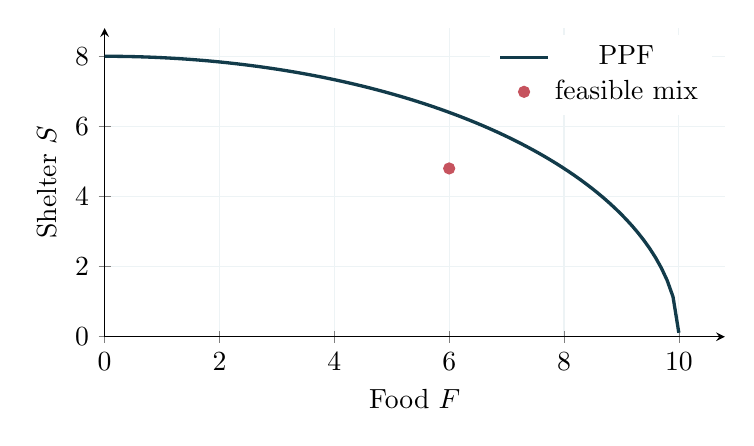
\begin{tikzpicture}
\begin{axis}[
  width=0.78\textwidth,height=5.5cm,
  axis lines=left,xlabel={Food $F$},ylabel={Shelter $S$},
  xmin=0,xmax=10.8,ymin=0,ymax=8.8,
  xtick={0,2,4,6,8,10},ytick={0,2,4,6,8},
  grid=major,grid style={econpale},
  legend style={draw=none,at={(0.98,0.98)},anchor=north east}
]
\addplot[domain=0:10,samples=100,very thick,color=econnavy] {8*sqrt(1-x^2/100)};
\addlegendentry{PPF}
\addplot[only marks,mark=*,color=econred] coordinates {(6,4.8)};
\addlegendentry{feasible mix}
\end{axis}
\end{tikzpicture}
\end{center}

\section{Absolute and comparative advantage}

A person or country has an \term{absolute advantage} in a task when it can produce more with the same inputs. \term{Comparative advantage} concerns opportunity cost. A party can have an absolute advantage in every activity and still gain from trade if opportunity costs differ.

Suppose Country A can produce either 10 units of food or 5 units of cloth per day. Country B can produce either 6 food or 4 cloth. A has an absolute advantage in both. The opportunity cost of one cloth is 2 food in A and 1.5 food in B. B has comparative advantage in cloth; A has comparative advantage in food. With voluntary exchange at a rate between 1.5 and 2 food per cloth, both can move beyond their own autarky consumption possibilities.

The model assumes that specialization is feasible, transport costs are small, preferences are compatible, and distribution can be addressed. Real trade generates winners and losers within countries. Gains from trade are not the same as gains for every worker, place, or firm.

\section{Marginal reasoning}

The \term{marginal} effect is the change from one more unit, holding the relevant comparison fixed. If total benefit from $q$ units is $B(q)$ and total cost is $C(q)$, the marginal benefit and marginal cost are approximately
\[
  MB(q)=\frac{\Delta B}{\Delta q},\qquad MC(q)=\frac{\Delta C}{\Delta q}.
\]
An interior optimum satisfies $MB=MC$ when both are smooth and the choice is divisible. This is a local condition, not a proof that the chosen quantity is globally best. Non-convex costs, fixed costs, strategic responses, and uncertainty can create multiple optima.

\section{Exercises}

\exercise{Country A produces 12 fish or 4 boats; Country B produces 10 fish or 5 boats. Who has comparative advantage in boats? Give a mutually beneficial terms of trade.}

\exercise{Why can an economy move inside its PPF even when its technology has not changed?}

\solution{The opportunity cost of one boat is 3 fish in A and 2 fish in B, so B has comparative advantage in boats. A trade ratio between 2 and 3 fish per boat can benefit both. An economy can move inside the frontier because of unemployment, coordination failure, conflict, illness, or unused capacity.}

\chapter{Supply, demand, and market equilibrium}
\label{ch:markets}

\section{Demand and supply}

A \term{demand curve} describes the quantities buyers would choose at different prices, holding other determinants fixed. A movement along the curve follows a price change. A shift occurs when income, tastes, expectations, prices of related goods, population, or information changes. A \term{supply curve} similarly describes sellers' intended quantities at different prices, holding technology, input prices, taxes, and expectations fixed.

For a linear illustration, let demand and supply be
\[
  Q_d=a-bP,\qquad Q_s=c+dP,
\]
where $Q$ is quantity, $P$ is price, $a$ and $c$ are intercept parameters, and $b,d>0$ are slope parameters. In a competitive market, an equilibrium satisfies $Q_d=Q_s$. Solving gives
\[
  P^*=\frac{a-c}{b+d},\qquad Q^*=\frac{ad+bc}{b+d}.
\]
For $a=120$, $b=2$, $c=20$, and $d=1$, the equilibrium is $P^*=33.33$ and $Q^*=53.33$. The supplied Python file reproduces the calculation and plots the curves.

\begin{center}
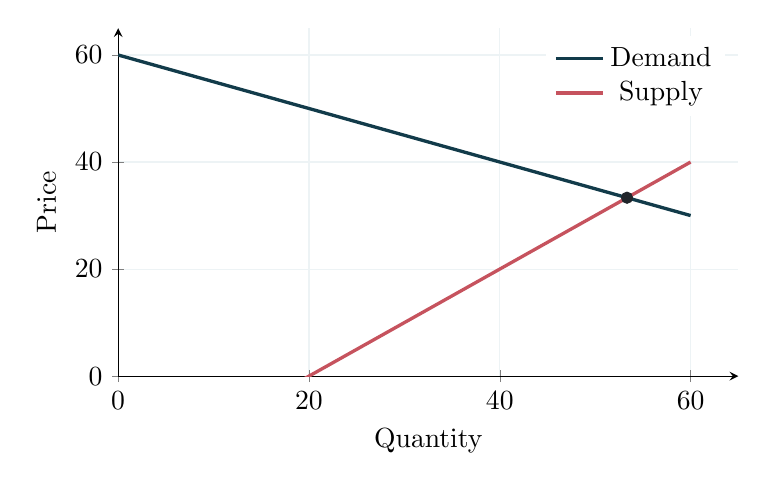
\begin{tikzpicture}
\begin{axis}[
  width=0.78\textwidth,height=6cm,
  axis lines=left,xlabel={Quantity},ylabel={Price},
  xmin=0,xmax=65,ymin=0,ymax=65,
  xtick={0,20,40,60},ytick={0,20,40,60},
  grid=major,grid style={econpale},
  legend style={draw=none,at={(0.98,0.98)},anchor=north east}
]
\addplot[domain=0:60,very thick,color=econnavy] {(120-x)/2};
\addlegendentry{Demand}
\addplot[domain=0:60,very thick,color=econred] {x-20};
\addlegendentry{Supply}
\addplot[only marks,mark=*,color=econink] coordinates {(53.3333,33.3333)};
\end{axis}
\end{tikzpicture}
\end{center}

\section{Elasticity}

\term{Elasticity} measures a percentage response to a percentage change. The price elasticity of demand is
\[
  \varepsilon_d=\frac{\%\,\text{change in }Q_d}{\%\,\text{change in }P}.
\]
Demand is called elastic when $|\varepsilon_d|>1$ and inelastic when $|\varepsilon_d|<1$. Elasticity is not the same as slope: percentage scaling means that the same curve can have different elasticity at different points. A firm raising price increases revenue when demand is locally inelastic, but the conclusion depends on the demand curve, competition, and reactions.

\section{Welfare and incidence}

\term{Consumer surplus} is the difference between a buyer's willingness to pay and the price paid, aggregated across units. \term{Producer surplus} is the difference between the price received and the minimum price at which sellers would supply, aggregated across units. In the simple competitive model, their sum is total surplus. A tax creates a wedge between the buyer price and seller price. The less elastic side of the market usually bears more of the tax burden, regardless of which side is legally charged.

This welfare language is conditional. It values benefits and costs through willingness to pay, which reflects income and existing rights. A policy can raise measured surplus while worsening distribution, dignity, health, political voice, or ecological stability. Distributional weights and rights must be made explicit rather than hidden inside an aggregate.

\section{Price controls}

A binding price ceiling below the market-clearing price creates excess demand in the basic model. A binding price floor above equilibrium creates excess supply. The model does not tell us how rationing occurs. Queues, search, discrimination, waiting, quality reduction, informal markets, and political allocation are all possible. Housing rent regulation therefore cannot be evaluated from the label alone: design, duration, coverage, supply response, tenant mobility, and complementary housing policy matter.

\section{Exercises}

\exercise{For $Q_d=100-2P$ and $Q_s=10+P$, find equilibrium price and quantity. If a tax of 9 per unit is placed on sellers, express the new seller and buyer prices.}

\exercise{Why can the legal assignment of a tax be irrelevant to its economic incidence in a competitive model?}

\solution{Equating quantities gives $100-2P=10+P$, so $P^*=30$ and $Q^*=40$. With a seller tax $t=9$, buyers pay $P_b$ and sellers receive $P_s=P_b-9$. Substitution gives $100-2P_b=10+(P_b-9)$, so $P_b=33$ and $P_s=24$, with $Q=34$. The less elastic side bears more because it changes quantity less in response to the wedge.}

\chapter{Consumers, firms, and the limits of optimization}
\label{ch:agents}

\section{Consumer choice}

The budget constraint in Chapter 1 defines what is affordable; preferences determine how affordable bundles are ranked. With utility $U(x,y)=x^\alpha y^{1-\alpha}$, where $0<\alpha<1$, a household with income $m$ and prices $p_x,p_y$ chooses
\[
  \max_{x,y}\ x^\alpha y^{1-\alpha}\quad\text{subject to}\quad p_xx+p_yy\leq m.
\]
For an interior solution, the Lagrange method gives
\[
  x^*=\frac{\alpha m}{p_x},\qquad y^*=\frac{(1-\alpha)m}{p_y}.
\]
The result says that the household spends a fixed share of income on each good in this particular preference model. It is not a universal law of consumption. Necessities, habits, durable goods, credit constraints, household bargaining, and uncertainty can produce different responses.

When the price of a good changes, the total change in demand can be divided into a \term{substitution effect} and an \term{income effect}. The substitution effect is the response to the changed relative price while compensating purchasing power; the income effect is the response to changed real purchasing power. For a normal good, a price increase generally lowers demand through both channels. For an inferior good, the income effect may work in the opposite direction. A Giffen response requires the income effect to dominate, a rare but theoretically possible case.

\section{Choice under risk}

Expected utility represents a risky lottery by
\[
  \E[U(w)]=\sum_{s=1}^{S}\pi_s U(w_s),
\]
where $\pi_s$ is the probability of state $s$ and $w_s$ is wealth in that state. Concavity of $U$ represents risk aversion: a certain amount can be preferred to a fair gamble with the same expected value. Insurance is valuable because it trades a small certain premium for protection against a large uncertain loss.

Expected utility is a benchmark, not a full psychology. Reference points, framing, probability weighting, ambiguity, and social comparison can matter. Behavioural models are most useful when they specify a mechanism that predicts departures from the benchmark and can be tested.

\section{Production and costs}

A firm transforms inputs into output. A production function $q=f(K,L)$ maps capital $K$ and labour $L$ into technically feasible output $q$. Under constant returns to scale, doubling both inputs doubles output. Diminishing marginal product of an input means that, holding other inputs fixed, an additional unit contributes less output than the previous one.

If a firm faces wage $w$ and rental price of capital $r$, its cost is $C=wL+rK$. Profit is
\[
  \pi(q)=p q-C(q),
\]
where $p$ is output price. A price-taking firm with differentiable cost chooses output where $p=MC(q)$ on the rising part of marginal cost, provided it is profitable to operate. The short-run supply curve can be derived from this condition, but fixed costs and shutdown decisions matter.

\section{Firms as organizations}

Ronald Coase asked why production is often coordinated inside firms rather than through a series of market contracts \cite{coase1937}. A firm can economize on search, bargaining, monitoring, and enforcement costs, but internal authority creates its own costs. Modern firms combine contracts, routines, culture, software, hierarchy, teams, and professional norms.

The \term{principal-agent problem} occurs when one party delegates a task and cannot perfectly observe the other's effort or information. Pay-for-performance can improve incentives but may also distort effort toward measured tasks, discourage cooperation, or induce gaming. A good contract therefore balances incentive intensity with risk sharing, measurability, and the value of discretion.

\section{Exercises}

\exercise{Use $U(x,y)=x^{1/2}y^{1/2}$, income $m=100$, and prices $p_x=5,p_y=2$. Find the demand for each good.}

\exercise{Why might a firm use a fixed salary rather than a pure commission even when sales are observable?}

\solution{The Cobb-Douglas formula gives $x^*=0.5(100)/5=10$ and $y^*=0.5(100)/2=25$. A fixed salary can insure a risk-averse worker against demand shocks, encourage non-measured tasks, reduce manipulation of sales metrics, and support team production.}

\chapter{Information, institutions, and economic power}
\label{ch:institutions}

\section{Information is costly and uneven}

Markets often work because participants can learn quality through experience, reputation, warranties, regulation, or repeated interaction. They can fail when one side knows more about quality or action than the other. In Akerlof's \term{lemons} model, buyers who cannot distinguish good and bad used cars offer a price based on average quality \cite{akerlof1970}. Owners of high-quality cars may withdraw, lowering average quality further. The mechanism is adverse selection: hidden information affects who enters a contract.

\term{Moral hazard} is different. After a contract is signed, effort or care may be unobserved, so insurance or a guarantee can change behaviour. Deductibles, monitoring, professional standards, and co-payment are possible responses; each has distributional and administrative costs.

\section{Signals and screening}

A \term{signal} is an action whose cost differs across types and therefore conveys information. Education can increase skills, signal persistence, or do both. A \term{screen} is a mechanism designed by the less-informed side, such as an application process, test, deductible, or menu of contracts. The empirical question is not whether a credential is ``really'' skill or signal in the abstract; it is how much of its payoff is caused by learning, selection, network access, legal status, or signalling in a particular institution.

\section{Property rights and transaction costs}

Property rights specify who may use an asset, receive its returns, exclude others, transfer it, and alter its condition. Clear rights can support investment, but formal title alone does not guarantee security, fair bargaining, or productive use. Enforcement can be private, communal, administrative, or judicial.

The Coasean insight is conditional: if bargaining is costless and rights are well defined, parties may reach an efficient arrangement regardless of the initial assignment of rights. In actual settings, transaction costs, power asymmetry, missing information, strategic delay, and wealth constraints matter. The initial legal allocation can therefore affect both efficiency and distribution.

\section{Commons and collective governance}

A common-pool resource is difficult to exclude people from using and is rival in use. Fisheries, groundwater, forests, and shared digital infrastructure can be overused, but outcomes are not predetermined. Elinor Ostrom's comparative work showed that communities sometimes develop monitoring, graduated sanctions, conflict-resolution, and locally legitimate rules \cite{ostrom1990,ostrom2010}. The relevant choice is not simply market versus state. Polycentric governance can combine household, community, municipal, national, and international rules.

\section{Power and institutional change}

Institutions persist because they coordinate expectations, distribute rents, and create constituencies that defend them. They can also change through crisis, conflict, technological change, demographic shifts, court decisions, social movements, or organized reform. North emphasized path dependence \cite{north1990}; institutional political economy asks who has the power to write, interpret, and enforce the rules. A growth-promoting reform can be politically blocked when it threatens incumbents, even if aggregate gains are large.

\begin{warningbox}
\textbf{Do not treat institutions as a residual.} Saying that ``institutions matter'' is a starting hypothesis. A useful explanation identifies the rule, the actors who enforce it, the incentives it creates, the distributional effects, and the mechanism linking it to observed outcomes.
\end{warningbox}

\section{Exercises}

\exercise{Give one example in which a warranty reduces adverse selection and one in which it reduces moral hazard. Explain the difference.}

\exercise{Why is a common resource not the same as a public good?}

\solution{A warranty can reveal seller confidence and attract high-quality products, reducing adverse selection. It can also motivate careful maintenance by excluding damage caused by misuse, reducing moral hazard. A public good is generally non-rival and difficult to exclude users from; a common-pool resource is rival, so one person's use reduces what remains for others.}

\chapter{Competition, monopoly, and strategic interaction}
\label{ch:competition}

\section{Market structure}

Perfect competition is a benchmark with many small firms, homogeneous products, free entry and exit, good information, and price-taking. Few real markets satisfy all assumptions. The benchmark is valuable because each relaxation highlights a specific mechanism.

A monopolist chooses quantity knowing that its demand curve slopes downward. Total revenue is $TR(q)=p(q)q$; marginal revenue is the change in revenue from one more unit. Profit maximization sets $MR=MC$, not $p=MC$. The markup depends on elasticity:
\[
  \frac{p-MC}{p}=\frac{1}{|\varepsilon_d|}
\]
under the standard monopoly model. A less elastic demand permits a larger markup, but entry threats, regulation, product quality, dynamic innovation, and multi-sided platforms complicate the inference.

\section{Oligopoly and game theory}

When a few firms interact, each must anticipate rivals. A \term{strategy} is a complete plan for responding to possible actions. A \term{Nash equilibrium} is a profile in which no player can improve its payoff by changing strategy alone, holding others fixed.

Consider a one-shot quantity game. Each of two firms chooses High or Low capacity, with payoffs:

\begin{center}
\begin{tabular}{lcc}
\toprule
 & Firm B: High & Firm B: Low\\
\midrule
Firm A: High & $(3,3)$ & $(1,5)$\\
Firm A: Low & $(5,1)$ & $(2,2)$\\
\bottomrule
\end{tabular}
\end{center}

The pair (Low, Low) is a Nash equilibrium if each firm prefers Low when the other chooses Low; the table does not make (High, High) an equilibrium, although different payoffs could. The table shows why strategic equilibrium is not the same as social optimum. Repeated interaction, reputation, communication, antitrust law, and technological change can alter the game.

\section{Entry, innovation, and platforms}

Market power can arise from scale economies, network effects, control of data, patents, switching costs, scarce locations, or regulation. A temporary monopoly can reward innovation and finance risky investment. It can also become durable through exclusion, acquisition, or control of essential interfaces. Competition policy therefore asks not only whether a price is high today but how market structure affects entry, quality, innovation, and political influence.

\section{Exercises}

\exercise{Explain why a monopolist's marginal revenue is below price when demand slopes downward.}

\exercise{Construct a two-player game in which a socially beneficial action is not a Nash equilibrium. Name one institution that could change the incentives.}

\solution{To sell one more unit, a monopolist must lower price on units it was already selling, so the added revenue is less than the new price. A public-goods contribution game has this property: each player free-rides on the other's contribution. Taxes, subsidies, enforceable agreements, or repeated-game norms can change the payoff structure.}

\chapter{Externalities, public goods, and public economics}
\label{ch:public}

\section{When private cost and social cost diverge}

An \term{externality} occurs when an action affects a third party outside the decision-maker's market transaction. With a negative production externality, marginal social cost is
\[
  MSC(q)=MPC(q)+MD(q),
\]
where $MPC$ is marginal private cost and $MD$ is marginal damage. The competitive quantity solves demand $=MPC$; the efficient quantity solves demand $=MSC$. A corrective tax equal to marginal damage at the efficient quantity is a Pigouvian benchmark. Measuring marginal damage is difficult, and the tax can be regressive unless paired with transfers.

\section{Public goods and collective action}

A \term{public good} is non-rival and non-excludable in the idealized definition. National defence is a common example, although actual public goods are often congestible or partially excludable. The free-rider problem means that voluntary private contributions may be below the socially preferred level. Political provision can solve coordination but introduces information, representation, and bureaucratic problems.

\term{Public choice} applies incentives and strategic reasoning to voters, officials, bureaucrats, regulators, and organized interests. It warns against assuming that the public sector automatically maximizes a benevolent social objective. The warning should not be inverted into a claim that markets automatically do so. Both systems require accountability, information, and contestable authority.

\section{Taxation and social welfare}

Taxes finance public goods, redistribute resources, correct externalities, and shape behaviour. A simple social welfare function is
\[
  W=\sum_{i=1}^{n}g_i U_i,
\]
where $U_i$ is the well-being of person $i$ and $g_i$ is a normative weight. The formula makes distributional priorities visible. Utilitarian weights may put greater value on transfers to people with low marginal utility of income, but other views emphasize rights, equality, capabilities, or sufficientarian thresholds.

The marginal cost of public funds includes the real resources needed to administer a tax and behavioural distortions, not merely the revenue transferred. Tax design should consider avoidance, evasion, incidence, labour supply, saving, investment, political feasibility, and the uses of revenue.

\section{Environment as an economic system}

A climate or ecosystem is not a single externality added to a standard model after the fact. It is a stock-flow system with thresholds, irreversibility, uncertainty, and intergenerational effects. Carbon pricing, standards, public investment, innovation policy, conservation, and adaptation can be complements. Discounting future benefits is an ethical and empirical choice, not a neutral technical detail.

\section{Exercises}

\exercise{A factory's private marginal cost is $20+q$ and marginal damage is $q$, while marginal benefit is $100-q$. Find the private and efficient quantities.}

\exercise{Why can a carbon tax be efficient in the model but politically difficult in practice?}

\solution{Private equilibrium satisfies $100-q=20+q$, so $q=40$. Social equilibrium satisfies $100-q=20+q+q$, so $q=26.67$. A carbon tax can impose visible costs before benefits arrive, affect regions and workers differently, be uncertain because damages are uncertain, and be distrusted if revenue use and compensation are unclear.}

\part{People, work, and distribution}

\chapter{Labour, education, health, and housing}
\label{ch:people}

\section{Labour is not an ordinary commodity}

Labour is a human activity embedded in bodies, households, identities, and law. A competitive labour-market model derives labour demand from the value of the marginal product and labour supply from the opportunity cost of time. It is a useful starting point, but workers do not move frictionlessly between jobs. Search costs, credentials, discrimination, geography, care responsibilities, collective bargaining, and employer concentration shape outcomes.

Under a simple production function $q=f(K,L)$, a competitive firm hires labour until
\[
  w=p\,MP_L,
\]
where $w$ is the wage, $p$ is output price, and $MP_L$ is the marginal product of labour. The equation is a condition within a model. It does not say that observed wages equal social value, because product markets can be imperfect, productivity can be jointly produced by teams and infrastructure, and bargaining can affect the division of surplus.

\section{Monopsony and institutions at work}

A monopsonist faces an upward-sloping labour supply curve because raising employment requires a higher wage. The marginal cost of labour then exceeds the wage paid to all workers, so employment and wages can be below the competitive benchmark. This gives a theoretical reason why a moderate wage floor or collective bargaining can increase both wages and employment in some settings. It does not imply that every wage floor has this effect; the result depends on demand, coverage, enforcement, substitution, and the size of the intervention.

The New Jersey and Pennsylvania fast-food study by Card and Krueger compared employment changes around a minimum-wage increase \cite{cardkrueger1994}. Their result challenged the simplest prediction of large employment losses. Reanalysis and later studies disputed some estimates, and the wider literature finds heterogeneous effects by worker group, sector, wage level, and design. The correct lesson is methodological: a textbook prediction is a testable hypothesis, not a substitute for identification and institutional detail.

\section{Education and human capital}

Education can raise productivity, provide social and civic capabilities, signal attributes, sort people into occupations, and change networks. A human-capital model treats schooling as an investment with costs today and expected benefits later. The return is not just a private wage premium; it may include health, participation, and effects on children. Nor does a correlation between schooling and earnings alone identify a causal return because ability, family resources, and selection may confound it.

Angrist and Krueger used quarter of birth as an instrument for schooling in the United States, exploiting compulsory-attendance rules \cite{angrist1991}. Their design illustrates both the power and the limits of instrumental variables: the estimate is tied to people whose schooling was changed by the instrument, and the exclusion and monotonicity assumptions require substantive defence.

\section{Health and care}

Health care has information asymmetry, uncertainty, externalities, urgent needs, and ethical constraints. Patients may not know which treatment is effective; providers may influence demand; insurers pool risks but can face selection; public health can generate benefits for others. These features explain why health systems commonly mix public finance, regulated providers, insurance, and private payment.

Care work, often unpaid or underpaid, sustains the labour force and human capabilities. A national account that excludes unpaid household production is not claiming that it has no value; it is applying a boundary designed for particular accounting purposes. Feminist economics asks how the boundary, the distribution of time, and the organization of care affect measured growth and lived welfare.

\section{Housing}

Housing is simultaneously consumption, location, an asset, a platform for care and education, and a source of collateral. Supply depends on land, planning, infrastructure, construction capacity, finance, and local political coalitions. Demand depends on income, household formation, amenities, expectations, and access to credit. Rents and prices can rise even when construction is increasing if demand grows faster or if new units are not close substitutes for existing stock.

Policies such as rent regulation, housing allowances, social housing, zoning reform, public land, and tenant protection act through different mechanisms. Evaluation should separate short-run distribution from long-run supply and neighbourhood effects rather than asking whether a policy is simply ``pro-market'' or ``anti-market.''

\section{Exercises}

\exercise{Why does a wage equal to marginal revenue product not imply that workers receive the whole value they help create?}

\exercise{List two reasons an education wage premium may not equal the causal effect of schooling.}

\solution{The firm may retain surplus because of market power, bargaining, property rights, or fixed factors. The premium may reflect ability, family background, networks, selection into education, or credential signalling rather than only skills acquired in school.}

\chapter{Inequality, poverty, mobility, and redistribution}
\label{ch:inequality}

\section{Different distributions answer different questions}

\term{Inequality} may concern income, wealth, consumption, health, education, time, power, or capabilities. The \term{Gini coefficient} summarizes dispersion in a distribution, but it does not identify who is poor, why inequality arose, or whether a given change improved well-being. Quantile ratios, percentile shares, poverty gaps, and mobility measures reveal different features.

Absolute poverty asks whether resources fall below a threshold; relative poverty compares resources with prevailing living standards; multidimensional poverty includes non-income deprivations. World Bank poverty estimates rely on household surveys, purchasing-power adjustments, and a defined poverty line \cite{wdi}. They are useful for global comparison but are not interchangeable with national poverty statistics or direct measures of lived deprivation.

\section{Income, wealth, and bargaining}

Income is a flow over a period; wealth is a stock of assets and liabilities. A household can have low current income but substantial wealth, or high income with little security. Inequality reflects market earnings, ownership, inheritance, taxes, transfers, discrimination, household composition, macroeconomic conditions, and political institutions.

A production model can explain a wage as a marginal product; a political-economy model asks who owns complementary assets, who sets rules, and how workers can contest them. Marxian analysis emphasizes class relations, exploitation, accumulation, and crisis. It offers concepts about ownership and power that are not reducible to preferences, while standard models offer precise tools for substitution, incidence, and constraints. The traditions can be compared by mechanisms rather than slogans.

\section{Redistribution}

Redistribution can occur before market income is formed, through education, labour law, health systems, property rules, and public infrastructure, or after market income, through taxes and transfers. A transfer may reduce poverty directly, insure against shocks, and improve bargaining power. It may also have administrative costs or behavioural responses. The existence of a response is not by itself a reason to reject a policy; it is part of measuring its net effect.

A simple tax schedule is progressive when the average tax rate rises with income. Progressivity can be measured on market income, disposable income, or consumption, producing different conclusions. Tax expenditures, payroll contributions, indirect taxes, and in-kind benefits must be included to compare systems.

\section{Mobility and opportunity}

Intergenerational mobility describes how a person's economic position relates to that of their parents. Chetty and co-authors used administrative earnings data to study mobility in the United States and showed that place is associated with large differences in outcomes \cite{chetty2014}; subsequent work studies mechanisms such as neighbourhood conditions, segregation, schools, social capital, and labour markets. Association across generations is not the same as a policy effect, and mobility can rise because both poor and rich outcomes worsen.

\section{Gender, care, and intersectionality}

Feminist economics treats the household as a site of bargaining rather than a single agent with a single interest. Time-use data reveal unpaid work and unequal exposure to care interruptions. Gender intersects with class, race, disability, migration status, age, and sexuality; averages can conceal sharply different constraints. A policy evaluation should therefore report heterogeneous effects when sample size and design permit.

\begin{keybox}
\textbf{Distributional checklist.} Identify the unit of analysis, the resource being measured, the time horizon, taxes and transfers included, household assumptions, and the counterfactual. Then ask how the policy changes voice, security, and exposure to risk, not only disposable income.
\end{keybox}

\section{Exercises}

\exercise{Give one example of a policy that changes market incomes before taxation and one that changes disposable income after taxation.}

\exercise{Why is a fall in the Gini coefficient not necessarily evidence that every household is better off?}

\solution{A stronger collective-bargaining regime can change wages before tax; a child benefit changes disposable income after tax. A Gini fall can occur because high incomes fell during a recession, because low incomes rose only slightly, or because non-income dimensions worsened. Distributional statistics require context.}

\chapter{Behavioural, experimental, and evolutionary economics}
\label{ch:behaviour}

\section{From rational choice to bounded rationality}

The standard model uses coherent preferences and optimization to generate sharp predictions. Herbert Simon argued that decision-makers face limited information, time, attention, and computational capacity \cite{simon1955}. They may \term{satisfice}: search until an option meets an aspiration level. This is not the absence of reasoning; it is reasoning under constraints.

Kahneman and Tversky's prospect theory models reference dependence, loss aversion, and non-linear probability weighting \cite{kahn1979}. People may evaluate a change relative to a status quo rather than final wealth, and the same outcome can be framed as a gain or a loss. These patterns are regular in many laboratory and field settings, but their magnitude and persistence depend on stakes, learning, culture, and institutional context.

\section{Social preferences and norms}

People often care about fairness, reciprocity, identity, status, and the welfare of others. A simple social-preference utility is
\[
  U_i=\pi_i-\alpha_i\max(\pi_j-\pi_i,0)-\beta_i\max(\pi_i-\pi_j,0),
\]
where $\pi_i$ and $\pi_j$ are payoffs and $\alpha_i,\beta_i\geq0$ capture sensitivity to disadvantageous and advantageous inequality. Such models explain why people may reject unequal offers, reward cooperation, or punish free-riding even at a private cost. They do not prove that one definition of fairness is universally correct.

\section{Experiments}

A laboratory experiment controls rules and observes decisions. A field experiment changes a policy in a real setting. Random assignment can identify an average causal effect for the study population when implementation and measurement are sound. Experiments can still have spillovers, demand effects, attrition, non-compliance, and limited external validity. Replication and pre-analysis reduce the risk that a striking result is an accident of a small sample or many tested outcomes.

\section{Evolutionary and institutional dynamics}

Evolutionary economics studies how routines, technologies, firms, and norms vary, are selected, and change. A replicator equation can be written
\[
  \dot{s}_i=s_i\left(\pi_i-\bar{\pi}\right),
\]
where $s_i$ is the share of type $i$, $\pi_i$ is its payoff, and $\bar{\pi}$ is the average payoff. Types that perform better grow in share in this simple model. Real economies also include invention, power, learning, imitation, lock-in, and deliberate institutional change.

\section{Exercises}

\exercise{Describe a choice for which a default might be useful and one for which it could be manipulative.}

\exercise{Why should a behavioural claim be tested in the institution where policy will be applied?}

\solution{Automatic pension enrolment can reduce inattention costs, while a hidden cancellation barrier can exploit inertia. Behaviour depends on stakes, information, social meaning, and available alternatives; a laboratory result may not transport to a workplace, clinic, or public service.}

\chapter{Firms, innovation, and the financial side of production}
\label{ch:firms}

\section{Why firms invest}

Investment creates productive capacity but is irreversible, uncertain, and sensitive to financing conditions. A simple net-present-value rule compares the present value of expected cash flows with the initial cost:
\[
  NPV=-I_0+\sum_{t=1}^{T}\frac{\E[CF_t]}{(1+r)^t},
\]
where $I_0$ is the initial investment, $CF_t$ is cash flow in period $t$, and $r$ is the discount rate. The rule is conditional on a known ownership structure, risk adjustment, tax system, and ability to finance. Real options matter because waiting can preserve the option to learn before committing.

\section{Innovation and productivity}

Innovation can lower costs, create products, reorganize work, or open markets. A patent can encourage disclosure and investment but grants temporary exclusion. Knowledge often has spillovers: firms cannot capture all benefits of research, creating a case for public funding or coordination. Schumpeterian analysis emphasizes creative destruction; endogenous-growth models emphasize ideas, human capital, and incentives. Neither implies that every new technology raises welfare for every group.

\section{Finance and agency}

Finance channels savings toward investment and provides payment, liquidity, risk sharing, and information. Banks transform maturities and monitor borrowers, but leverage makes them fragile. Limited liability supports risk taking and entrepreneurship but can create moral hazard. Corporate governance asks how owners, managers, workers, creditors, and communities share control and risk.

\section{Exercises}

\exercise{An investment costs 100 today and pays 60 in each of the next two years. At a discount rate of 10 percent, calculate its NPV.}

\exercise{Why can a patent both encourage and impede innovation?}

\solution{$NPV=-100+60/1.1+60/1.1^2\approx3.31$, so it is positive under the stated assumptions. A patent rewards invention and disclosure, but exclusion can raise prices, block follow-on innovation, and create strategic patent thickets.}

\part{Macroeconomics and the economic system}

\chapter{National accounts and macroeconomic measurement}
\label{ch:accounts}

\section{The circular flow}

Macroeconomics studies aggregates and interactions among households, firms, governments, financial institutions, and the rest of the world. National accounts organize flows of production, income, expenditure, saving, and finance. The circular flow is an accounting map, not a complete causal theory.

For a closed economy with government, expenditure on final output can be written
\[
  Y=C+I+G,
\]
where $Y$ is gross domestic product, $C$ household consumption, $I$ investment, and $G$ government purchases of final goods and services. With trade,
\[
  Y=C+I+G+NX,\qquad NX=X-M,
\]
where $X$ is exports and $M$ imports. This is an accounting identity: it holds by construction for the defined aggregates. It does not imply that an increase in $G$ must raise $Y$ by the same amount.

From the income side, production generates compensation, operating surplus, taxes less subsidies, and depreciation adjustments. In principle, GDP measured by expenditure, income, and production coincide. In practice, independent data sources create statistical discrepancies and revisions. The U.S. BEA's NIPA Handbook explains the concepts and methods behind these accounts \cite{bea2025}; other countries use national versions of the System of National Accounts.

\section{Nominal, real, and per-capita measures}

Nominal GDP values output at current prices. Real GDP values output using a chain or fixed-price method intended to separate quantities from prices. A GDP deflator is
\[
  \text{deflator}=100\times\frac{\text{nominal GDP}}{\text{real GDP}}.
\]
Per-capita output divides an aggregate by population, but it is not the same as median income, household consumption, or well-being. GDP excludes or imperfectly measures unpaid care, leisure, distribution, environmental degradation, informal production, and quality changes.

\section{Inflation and unemployment}

The inflation rate is a percentage change in a price index. A consumer price index tracks the cost of a defined consumption basket; it can differ from the GDP deflator because the baskets and coverage differ. Index-number choices, substitution, quality adjustment, housing treatment, and sampling matter.

The ILO's strict unemployment concept counts working-age people without work who are available and actively seeking work during a reference period \cite{ilo}. The unemployment rate is unemployed divided by the labour force, not by the whole population. Broader underutilization measures include potential labour force and time-related underemployment. A falling unemployment rate can therefore reflect employment growth, labour-force exit, or both.

\section{Stocks, flows, and identities}

Debt is a stock; borrowing is a flow. A government's budget identity can be represented as
\[
  \Delta B=G-T+rB,
\]
where $B$ is debt, $G$ purchases and transfers as defined, $T$ revenue, and $rB$ interest spending. The exact sign convention and treatment of inflation, assets, and valuation changes matter. Identities organize data; they do not by themselves identify a behavioural response.

\section{Exercises}

\exercise{If nominal GDP rises by 8 percent while the GDP deflator rises by 3 percent, is real GDP growth exactly 5 percent? Give the approximation and the reason for the difference.}

\exercise{Why can a lower unemployment rate coincide with a weaker labour market?}

\solution{The common approximation is real growth of about 5 percent, but exact real growth depends on the index-number formula and interaction of price and quantity changes. Unemployment can fall because people leave the labour force or stop searching, so participation and employment must also be examined.}

\chapter{Growth, productivity, technology, and demography}
\label{ch:growth}

\section{The Solow model}

Long-run growth asks why productive capacity rises. In the basic Solow model, output is
\[
  Y=F(K,AL),
\]
where $K$ is physical capital, $L$ labour, and $A$ labour-augmenting technology. With constant returns, divide by effective labour $AL$ to obtain $y=f(k)$, where $k=K/(AL)$ and $y=Y/(AL)$. Capital per effective worker evolves as
\[
  \dot{k}=s f(k)-(\delta+n+g)k,
\]
where $s$ is the saving/investment rate, $\delta$ depreciation, $n$ population growth, and $g$ technological growth.

At a steady state, $\dot{k}=0$ \cite{solow1956}:
\[
  s f(k^*)=(\delta+n+g)k^*.
\]
For a Cobb-Douglas production function $f(k)=k^\alpha$, with $0<\alpha<1$,
\[
  k^*=\left(\frac{s}{\delta+n+g}\right)^{1/(1-\alpha)}.
\]
Higher saving raises the steady-state level of output per effective worker, but in the standard model it does not permanently raise the long-run growth rate unless it changes technology or population dynamics. The model highlights diminishing returns and the importance of productivity; it leaves the origin of $g$ outside the model.

\section{Productivity and institutions}

Productivity is output per input. Total factor productivity is a residual measure: it captures technology, organization, measurement error, utilization, and omitted inputs. It should not be read as a pure measure of ingenuity. Institutions affect investment security, competition, education, infrastructure, innovation, and the distribution of rents. Acemoglu, Johnson, and Robinson's institutional argument is influential but contested \cite{acemoglu2001,albouy2012}; the settler-mortality instrument and data have been criticized, including by Albouy. The appropriate conclusion is that historical institutions are an important hypothesis supported by some evidence, not a monocausal verdict.

\section{Demography}

Population ageing changes the ratio of dependants to workers, saving patterns, health demand, public budgets, and the composition of consumption. Migration can change labour supply, innovation, fiscal balances, and local housing demand. Demography is not destiny: participation, productivity, care systems, retirement rules, and technology mediate its economic effects. UN population projections are scenarios conditional on fertility, mortality, and migration assumptions, not precise prophecies \cite{un2024}.

\section{Growth traditions}

Classical political economy emphasized distribution among wages, profits, and rents. Neoclassical growth models emphasize accumulation and substitution. Keynesian and post-Keynesian approaches stress demand, uncertainty, financial instability, and path dependence. Schumpeterian and evolutionary approaches emphasize innovation and structural change; endogenous-growth theory models ideas and knowledge spillovers more explicitly \cite{romer1990}. Institutional and development economics focus on law, state capacity, power, and historical trajectories. Ecological economics asks whether indefinite material growth is compatible with finite biophysical systems.

\section{Exercises}

\exercise{With $s=0.20$, $\delta=0.05$, $n=0.02$, $g=0$, and $\alpha=1/3$, calculate the Solow steady-state $k^*$.}

\exercise{Why does higher saving not necessarily create permanently faster per-worker growth in the basic Solow model?}

\solution{$k^*=(0.20/0.07)^{3/2}\approx4.33$. Diminishing returns mean that extra capital raises the level of output but the economy eventually returns to a steady growth path determined by exogenous technology in the model.}

\chapter{Employment, inflation, and business cycles}
\label{ch:cycles}

\section{Short-run demand}

In the Keynesian cross, planned expenditure is \cite{keynes1936}
\[
  E=C(Y-T)+I+G+NX,
\]
where consumption depends on disposable income $Y-T$. Equilibrium output satisfies $Y=E$. With $C=a+c(Y-T)$ and fixed $I,G,NX,T$, the simple multiplier is
\[
  \frac{\partial Y}{\partial G}=\frac{1}{1-c}.
\]
The result depends on unused capacity, prices, imports, interest rates, expectations, taxes, and monetary policy. It is not a mechanical law in a fully employed economy.

Keynesian analysis emphasizes that aggregate demand can be insufficient and that uncertainty can depress investment. Classical and new classical traditions emphasize market clearing, intertemporal substitution, expectations, and supply-side constraints. New Keynesian models combine optimizing foundations with nominal rigidities and monetary policy. Post-Keynesian and financial-instability approaches give a larger role to credit, balance sheets, and endogenous crises \cite{minsky1986}.

\section{Inflation dynamics}

A stylized Phillips curve relates inflation to expected inflation, resource slack, and supply shocks:
\[
  \pi_t=\E_t\pi_{t+1}-\kappa(u_t-u^*)+v_t,
\]
where $\pi_t$ is inflation, $u_t$ unemployment, $u^*$ a reference rate, $\kappa>0$, and $v_t$ a supply shock. The equation is a model of conditional association, not a stable menu between inflation and unemployment. Expectations, credibility, labour-market institutions, and the time horizon matter.

\section{Business cycles}

A recession can arise from demand shocks, supply shocks, financial amplification, policy error, sectoral reallocation, conflict, or interacting mechanisms. Aggregate statistics can hide large differences across households and regions. A central analytical distinction is between a shock, the propagation mechanism, and the policy response.

\section{Forecasts and uncertainty}

Forecasts are conditional statements about a future path given a model, data, and assumptions. Prediction intervals should widen with horizon and parameter uncertainty. A forecast can be useful even when it is not exact; a precise point estimate can be harmful when uncertainty is suppressed. Scenario analysis is often more honest for structural breaks, climate risk, war, and new technology.

\section{Exercises}

\exercise{If the marginal propensity to consume is $c=0.75$, what is the simple government-spending multiplier? State one reason it may be smaller in an open economy.}

\exercise{Why can a supply shock raise inflation and unemployment at the same time?}

\solution{The multiplier is $1/(1-0.75)=4$. Imports, taxes, interest-rate responses, and capacity constraints reduce the realized multiplier. A negative supply shock shifts the short-run aggregate supply curve left: prices rise while output and employment fall.}

\chapter{Money, banking, central banks, and financial crises}
\label{ch:money}

\section{What money does}

Money functions as a medium of exchange, unit of account, and store of value. Modern money is largely a layered institutional claim: central-bank liabilities, commercial-bank deposits, and settlement arrangements. Its acceptability depends on law, trust, payment networks, convertibility, and expectations.

Banks accept deposits or other funding and make loans, transforming maturities and screening borrowers. A bank's balance sheet can be summarized as assets (loans and securities) equal to liabilities (deposits and borrowing) plus equity. Liquidity risk arises when short-term claims must be met before long-term assets mature; solvency risk arises when asset values are insufficient to cover liabilities.

\section{Central-bank policy}

Central banks influence short-term interest rates and financial conditions through policy rates, asset operations, lending facilities, reserve systems, and communication. The Federal Reserve describes its statutory goals as maximum employment, stable prices, and moderate long-term interest rates; other central banks have different mandates \cite{federalreserve}. Monetary policy transmission runs through borrowing costs, asset prices, exchange rates, expectations, and bank lending. The lag and strength are uncertain.

\section{Credit creation and constraints}

The simple money multiplier story is pedagogically useful but incomplete. In modern banking, loans create deposits, while lending is constrained by capital, liquidity, profitability, regulation, credit demand, risk, and settlement. Central-bank reserves are not mechanically multiplied into a fixed multiple of deposits. The institutional details differ across monetary systems.

\section{Financial crises}

A crisis can develop through leverage, maturity mismatch, asset-price feedback, correlated exposures, runs, opaque instruments, and procyclical regulation. A bank run is individually rational when each depositor fears others will withdraw, even if collective withdrawal destroys a solvent institution. Deposit insurance and lender-of-last-resort facilities can stop runs but create moral hazard, requiring supervision and credible resolution.

Hyman Minsky's financial-instability hypothesis emphasizes that long periods of stability can encourage riskier financing structures \cite{minsky1986}. Bernanke's historical analysis of the Great Depression highlighted how financial disruption can impair credit intermediation and amplify real contraction \cite{bernanke1983}. The 2007--09 global financial crisis demonstrated that systemic risk can arise outside traditional deposit banks through securitization, wholesale funding, and interconnected balance sheets.

\begin{warningbox}
\textbf{A crisis is not simply a market failure or a government failure.} Diagnose the balance sheets, incentives, legal structure, information, and political constraints. Rescue design determines who bears losses and whether future risk taking is encouraged.
\end{warningbox}

\section{Exercises}

\exercise{Explain the difference between liquidity and solvency risk. Give one policy that addresses each.}

\exercise{Why is deposit insurance usually paired with bank supervision?}

\solution{A liquid institution can meet short-term payments but may have assets whose value is below liabilities, while an illiquid institution may be solvent but unable to obtain cash quickly. Central-bank liquidity lending addresses the latter; capital rules and resolution address solvency. Insurance prevents runs but can reduce depositor monitoring, so supervision and risk-based rules limit moral hazard.}

\chapter{Fiscal policy, debt, and stabilization}
\label{ch:fiscal}

\section{Automatic and discretionary policy}

Fiscal policy includes public purchases, transfers, taxes, borrowing, and public investment. Automatic stabilizers such as progressive taxes and unemployment insurance respond to the cycle without a new legislative decision. Discretionary measures can target a shock but may arrive late or be distorted by political incentives.

The effect of fiscal policy depends on the state of the economy. When unemployment is high and monetary policy is constrained, public spending can raise demand and preserve productive relationships. Near capacity, the same spending can raise inflation or crowd out private activity. Public investment can also change long-run supply, but only if projects are useful, maintained, and competently delivered.

\section{Debt sustainability}

Let $b_t$ be debt as a share of GDP, $r$ the effective nominal interest rate, $g$ nominal GDP growth, and $pb_t$ the primary balance as a share of GDP, positive for a surplus. A stylized debt equation is
\[
  b_t=\frac{1+r}{1+g}b_{t-1}-pb_t.
\]
Debt can stabilize with a primary surplus, rapid nominal growth, or an interest rate below growth, but these conditions are not guaranteed. Sustainability is not a single debt ratio. It depends on the maturity structure, currency, investor base, fiscal institutions, growth, inflation, contingent liabilities, and the state's ability to tax.

\section{Austerity and policy disagreement}

Keynesian arguments warn that simultaneous spending cuts during a downturn can reduce demand and worsen debt ratios. Fiscal-conservative arguments stress credibility, intertemporal limits, tax distortions, and the risk that temporary measures become permanent. The empirical effect of consolidation depends on timing, composition, monetary response, exchange regime, household expectations, and international conditions. A slogan about multipliers cannot replace a model and evidence for the case at hand.

\section{Public investment and distribution}

Fiscal choices allocate risks across generations and groups. A bridge, school, benefit, tax credit, or debt write-down can have different effects by location, age, wealth, gender, and employment status. Cost-benefit analysis should report distributional incidence, not only a discounted aggregate net benefit. Where rights or thresholds are at stake, a pure willingness-to-pay sum may be inappropriate.

\section{Exercises}

\exercise{If $b_{t-1}=0.80$, $r=0.04$, $g=0.05$, and the primary balance is zero, calculate $b_t$.}

\exercise{Why can a fiscal expansion have a larger effect during a recession than during a boom?}

\solution{$b_t=(1.04/1.05)0.80\approx0.792$. The ratio falls slightly because nominal GDP grows faster than the interest rate. During a recession there may be idle resources, weaker private demand, and monetary policy at its effective lower bound, so public spending can displace less private activity.}

\chapter{Trade, exchange rates, and globalization}
\label{ch:trade}

\section{Why trade occurs}

Trade can reflect comparative advantage, economies of scale, product variety, technology differences, factor endowments, and historical networks. A tariff raises the domestic price above the world price in a small-country model, increases domestic production, reduces consumption, and creates tariff revenue. The standard deadweight-loss triangles quantify efficiency costs under strong assumptions.

Trade theory has expanded from comparative advantage to firm heterogeneity. Melitz's model shows that opening to trade can reallocate market share toward more productive firms while exposing less productive firms to exit \cite{melitz2003}. Consumers may gain from variety and lower prices, but workers and communities can face concentrated adjustment costs. Compensation, mobility, regional policy, and the speed of adjustment determine whether aggregate gains become broadly shared.

\section{Balance of payments}

The current account records trade in goods and services, primary income, and transfers. The financial account records cross-border asset transactions. With valuation changes and statistical discrepancies, the balance of payments accounts must reconcile. A current-account deficit is not automatically a crisis: it may finance productive investment, but it can also reflect unsustainable borrowing, asset-price booms, or weak domestic demand.

\section{Exchange rates}

The nominal exchange rate is the price of one currency in another. A real exchange rate adjusts for price levels and indicates the relative price of domestic and foreign goods. Depreciation can improve competitiveness, but the effect depends on import content, contracts, pass-through, demand elasticities, and foreign responses. The ``impossible trinity'' describes a tension among a fixed exchange rate, free capital mobility, and independent monetary policy: a country cannot fully maintain all three simultaneously.

\section{Capital flows and globalization}

Foreign direct investment can bring capital, technology, market access, and management practices; it can also create dependence, profit repatriation, or bargaining conflicts. Global value chains distribute production across borders, making firms productive and vulnerable at once. Financial globalization can diversify risk but transmit shocks quickly.

International institutions shape the rules of trade, debt, taxation, labour, and intellectual property. The relevant question is not whether globalization is ``good'' in the aggregate but who can exit, who absorbs shocks, and which domestic institutions convert gains into security and capability.

\section{Exercises}

\exercise{Name one gain and one adjustment cost of a tariff reduction. Why might both occur in the same country?}

\exercise{Why is a current-account deficit not equivalent to a government budget deficit?}

\solution{Consumers may get lower prices and more variety, while import-competing workers or firms lose market share. The gains and losses occur through different sectors and regions. The current account concerns cross-border trade and income; the government budget concerns public revenue, spending, and borrowing. They can interact but are not the same identity.}

\chapter{Development, institutions, technology, and economic history}
\label{ch:development}

\section{Development is multidimensional}

Development includes material living standards, health, education, security, agency, political inclusion, and ecological sustainability. GDP per person is informative but incomplete. Amartya Sen's capability approach asks what people are able to be and do, not only what commodities they possess \cite{sen1999}.

\section{Diverse paths}

The Industrial Revolution combined energy, mechanization, science, organization, markets, imperial relations, and political change. Its benefits were uneven and often depended on coercive labour and colonial extraction. Later development paths included state-led industrialization, export-oriented manufacturing, resource dependence, socialist planning, mixed economies, and service-led growth. There is no single institutional sequence that every country must reproduce.

\section{Institutions and causality}

Institutions may affect growth through property security, public goods, taxation, conflict management, innovation, and accountability. But institutional measures are endogenous: prosperous countries may build better institutions, and both may be caused by geography, history, social structure, or international power. Natural experiments, historical instruments, comparative case studies, and process tracing can complement cross-country regressions.

Acemoglu, Johnson, and Robinson's colonial analysis linked historical disease environments, settlement patterns, institutions, and present income \cite{acemoglu2001,albouy2012}. The contribution is an explicit causal strategy; the limitation is that the instrument's validity, data construction, and mechanisms remain contested. A mature reading treats the study as evidence within an argument, not as a final answer to why countries differ.

\section{Technology and structural transformation}

Development commonly involves movement from agriculture toward manufacturing and services, but the sequence varies. Technology can bypass stages, as mobile payments can reduce reliance on fixed-line banking. Adoption depends on complementary skills, infrastructure, finance, regulation, and demand. Productivity gains can coexist with precarious work if bargaining institutions do not share the surplus.

\section{Political economy}

States are not external to markets. They define property, build infrastructure, tax, educate, regulate, borrow, and sometimes own firms. Markets can discipline state firms, while states can coordinate investment that markets alone cannot finance. The quality of the state depends on capacity, legitimacy, representation, and checks on arbitrary power. Development policy is therefore an institutional design problem under political constraints.

\section{Exercises}

\exercise{Why can a country have rising GDP per capita but worsening capabilities for some groups?}

\exercise{Give one reason cross-country correlations between institutions and income may not identify the effect of institutions.}

\solution{Growth may accrue to a narrow sector while health, education, security, or environmental quality deteriorate for others. Reverse causality, omitted history, measurement error, and selective colonial or geographic processes can confound the correlation.}

\chapter{Ecological economics, climate, and the material economy}
\label{ch:ecology}

\section{The economy is embedded in nature}

Economic production uses energy and materials and generates waste. A flow of extraction can reduce a stock of natural capital; an emission flow can accumulate in the atmosphere. Conventional national accounts record many market transactions but not all changes in ecological stocks or irreversible damage.

An elementary carbon stock equation is
\[
  S_{t+1}=S_t+E_t-A_t,
\]
where $S_t$ is the atmospheric stock of carbon dioxide equivalent, $E_t$ emissions, and $A_t$ absorption. The equation makes clear why a flow reduction and a stock stabilization are different targets. Net-zero emissions means the flow is approximately balanced; it does not restore the stock automatically.

\section{Valuation and uncertainty}

Climate damages are uncertain, correlated across regions, and potentially nonlinear \cite{ipcc2023}. A social cost of carbon estimate depends on climate sensitivity, damage functions, discounting, adaptation, distributional weights, and the policy baseline. A single number can be useful for a decision rule but should be presented with assumptions and sensitivity ranges.

\section{Policy instruments}

A carbon tax uses prices to make emissions costly. A cap-and-trade system fixes a quantity and lets a permit price emerge. Standards can address information, coordination, or political constraints. Public research and infrastructure can lower the cost of clean alternatives. Adaptation reduces harm but does not remove the need for mitigation. Effective climate policy usually combines instruments and addresses distribution through rebates, public investment, labour transition, and international finance.

\section{Ecological and feminist critiques}

Ecological economics challenges the idea that all losses can be substituted by money and asks whether the scale of the economy fits biophysical limits. Feminist economics emphasizes social reproduction and unpaid care as material conditions of production. Both critiques broaden the object of economics without rejecting measurement, incentives, or institutional analysis.

\section{Exercises}

\exercise{If emissions are 100 units per year and absorption is 60, what happens to the stock after one year? What would stabilize the stock?}

\exercise{Why can a technology subsidy complement rather than replace a carbon price?}

\solution{The stock rises by 40 units, assuming other terms are zero. Stabilization requires emissions to fall to absorption, or absorption to rise to emissions, subject to measurement and permanence. A subsidy can reduce the cost and political burden of clean alternatives, while a carbon price changes incentives across technologies and uses.}

\chapter{Contemporary debates and unresolved questions}
\label{ch:debates}

\section{Automation and artificial intelligence}

New technologies can substitute for tasks, complement workers, create new tasks, lower costs, and change the distribution of bargaining power. The effects depend on adoption, organizational redesign, skills, ownership, labour institutions, and demand. Historical analogies are informative but not decisive. The right empirical unit is often the task or occupation within an institution, not ``technology'' as a single shock.

\section{Productivity and well-being}

Digital services, unpaid work, quality improvements, and environmental costs are difficult to measure. A productivity slowdown may reflect mismeasurement, weak diffusion, low investment, market concentration, demographic change, or a genuine fall in innovation. A well-being dashboard should not replace GDP with one new index; it should expose multiple dimensions and their trade-offs.

\section{Housing, inequality, and political legitimacy}

High housing costs can be symptoms of land scarcity, planning constraints, financialization, construction bottlenecks, or demand concentration. Inequality can weaken political trust when people perceive rules as rigged, but the relationship is mediated by institutions and narratives. Redistribution without supply, public capacity, or democratic legitimacy may be unstable; supply reforms without distributional protection may be unjust or politically impossible.

\section{Inflation, debt, and the state}

The inflation of the early 2020s renewed arguments about supply shocks, fiscal demand, labour markets, markups, expectations, and monetary policy. The general lesson is not that one school ``won.'' Inflation episodes combine mechanisms, and policy must distinguish temporary relative-price changes from persistent nominal dynamics. High debt can be sustainable under some conditions and destabilizing under others.

\section{Pluralism and what remains unknown}

Economics still lacks complete answers to questions about productivity, inequality, climate risk, political capture, long-run growth, financial instability, and the welfare effects of emerging technologies. Pluralism is not the claim that all theories are equally supported. It is a method of using rival models to expose assumptions, test mechanisms, and identify what evidence would change a conclusion.

\begin{keybox}
\textbf{A defensible economic conclusion has four parts:} a defined outcome; a causal or accounting mechanism; evidence appropriate to the claim; and a statement of external validity, distribution, and uncertainty.
\end{keybox}

\section{Exercises}

\exercise{Choose a current economic debate and separate one accounting identity, one empirical claim, one model assumption, one forecast, and one normative judgment.}

\exercise{Why should a policy report distinguish average effects from distributional effects?}

\solution{An identity describes how quantities must add up, while an empirical claim depends on data and identification. A model assumption is a conditional simplification; a forecast is a statement about an uncertain future; a normative judgment evaluates outcomes. Average gains can coexist with concentrated losses, so distribution determines political and ethical consequences.}

\part{Evidence, econometrics, and policy evaluation}

\chapter{Data, probability, and statistical reasoning}
\label{ch:data}

\section{Variables and measurement}

A variable records a feature that can differ across units or time. A dataset has observations (rows), variables (columns), and a data-generating process. A measure is not the object itself. GDP, income, health, trust, productivity, and poverty all require definitions, sampling, coding, and decisions about missing information.

Distinguish a population from a sample. A population is the set about which a claim is intended; a sample is the observed subset. A parameter describes the population; a statistic describes the sample. Sampling uncertainty is only one source of uncertainty. Measurement error, non-response, attrition, selection, model dependence, and data processing can matter as much.

\section{Probability}

Probability represents uncertainty about events. For an event $A$, $0\leq\Prob(A)\leq1$. Conditional probability is
\[
  \Prob(A\mid B)=\frac{\Prob(A\cap B)}{\Prob(B)},
\]
provided $\Prob(B)>0$. Independence means $\Prob(A\mid B)=\Prob(A)$, a strong assumption rather than a default.

A random variable $X$ takes numerical values. Its expectation is a probability-weighted average:
\[
  \E[X]=\sum_x x\Prob(X=x)
\]
for a discrete variable. Variance measures dispersion around the expectation:
\[
  \operatorname{Var}(X)=\E[(X-\E[X])^2].
\]

\section{Descriptive statistics}

The mean is sensitive to extreme values; the median is the middle observation after sorting; quantiles describe positions in a distribution. A histogram shows observations by bins, while a scatter plot shows relationships between two variables. Visualization should reveal missingness, outliers, scale, and heterogeneity rather than merely decorate a result.

The sample mean is $\bar{x}=n^{-1}\sum_i x_i$. The standard error of the mean is approximately $s/\sqrt{n}$ under independent sampling, where $s$ is the sample standard deviation. Clustering, serial correlation, and survey weights change this calculation.

\section{Correlation and regression}

The correlation coefficient standardizes covariance:
\[
  \rho_{XY}=\frac{\operatorname{Cov}(X,Y)}{\sigma_X\sigma_Y}.
\]
It describes linear association, not causation. A linear regression writes
\[
  Y_i=\beta_0+\beta_1X_i+u_i,
\]
where $u_i$ collects unexplained determinants. Ordinary least squares chooses coefficients that minimize the sum of squared residuals. In a one-regressor model, $\hat{\beta}_1$ is the change in predicted $Y$ associated with a one-unit change in $X$ in the sample.

The causal interpretation requires assumptions. If $X$ is correlated with omitted determinants in $u$, the coefficient combines a causal effect with confounding. Measurement error in $X$ can attenuate the coefficient in simple cases. Functional-form choices and heterogeneous effects can make a single slope misleading.

\section{Uncertainty and inference}

A confidence interval is a procedure with a long-run coverage property under repeated sampling and a specified model. It is not a probability statement that a fixed parameter lies in the particular interval. A p-value is the probability, under a null model, of data at least as incompatible with that model as the observed data; it is not the probability that the null is true.

Statistical significance does not measure substantive importance. Report effect sizes, uncertainty intervals, units, sample size, outcome definitions, and plausible alternative specifications. Correcting for many comparisons, preregistering outcomes, and making code available can reduce false discoveries.

\section{Exercises}

\exercise{A sample mean is 10 and the sample standard deviation is 4 for $n=100$ independent observations. What is the approximate standard error?}

\exercise{Give an example of a confounder in a regression of earnings on education.}

\solution{The standard error is $4/\sqrt{100}=0.4$. Family resources or prior ability can affect both education and earnings, so the education coefficient may not be causal without a design or credible adjustment.}

\chapter{Causal inference and econometrics}
\label{ch:causal}

\section{The counterfactual problem}

For person $i$, let $Y_i(1)$ be the outcome under treatment and $Y_i(0)$ the outcome without treatment. The individual causal effect is $Y_i(1)-Y_i(0)$, but only one potential outcome is observed. The average treatment effect is
\[
  ATE=\E[Y(1)-Y(0)].
\]
The core challenge is constructing a credible counterfactual for the observed treated group.

\section{Randomized experiments}

Random assignment makes treatment statistically independent of potential outcomes in expectation. The difference in mean outcomes estimates the ATE when compliance, attrition, interference, and measurement are handled \cite{imbensrubin2015}. If some assigned participants do not take treatment, the intention-to-treat effect remains the effect of assignment. Instrumental-variable estimates can identify a local average treatment effect for compliers under exclusion and monotonicity.

\section{Observational designs}

Matching attempts to compare treated and untreated units with similar observed covariates. It cannot solve unmeasured confounding without assumptions. Difference-in-differences compares changes over time between treated and comparison groups:
\[
  \widehat{\tau}_{DID}=(\bar{Y}_{T,post}-\bar{Y}_{T,pre})-(\bar{Y}_{C,post}-\bar{Y}_{C,pre}).
\]
The key parallel-trends assumption is that, without treatment, the groups would have changed similarly. Pre-trends are informative but cannot prove future parallel trends.

Regression discontinuity uses a treatment rule at a cutoff in a running variable. It identifies a local effect if units cannot precisely manipulate the cutoff and potential outcomes are continuous at the threshold. Instrumental variables use a variable that shifts treatment but affects the outcome only through treatment; the exclusion restriction is usually the hardest part to defend. The broader warning is the Lucas critique: policy changes can alter expectations and behaviour, so historical reduced-form relationships need not remain invariant under a new regime \cite{lucas1976}.

\section{Heterogeneity and external validity}

An average effect can hide benefits for one group and harm for another. Report treatment effects by baseline risk, income, gender, age, place, and implementation when pre-specified and statistically credible. External validity asks whether the mechanism, treatment, population, outcome, and institutional context travel. A precise local estimate may be more credible than a broad generalization.

\section{Forecasting and structural models}

Forecasting evaluates predictive performance, often using out-of-sample tests, rolling windows, and proper scoring rules. Causal policy analysis asks what would happen under an intervention, which can require a structural model of behaviour and equilibrium responses. A model can forecast well without identifying a policy effect, and a causal estimate can be useful even when it is not a good long-run forecast.

\section{A transparent workflow}

\begin{enumerate}
  \item Define the estimand, population, treatment, outcome, and time horizon.
  \item Draw the causal story, including plausible confounders and mediators.
  \item Inspect data provenance, missingness, coding, timing, and measurement.
  \item Choose a design that addresses the main threat, not the easiest regression.
  \item Pre-specify primary outcomes and robustness checks when possible.
  \item Report the estimate, uncertainty, assumptions, failures, and limits.
  \item Test whether the mechanism survives alternative samples, periods, and institutions.
\end{enumerate}

The supplied difference-in-differences script uses simulated data with a known treatment interaction. It demonstrates arithmetic, not an empirical finding. The fact that a regression produces a coefficient does not make the coefficient causal.

\section{Exercises}

\exercise{In a difference-in-differences study, why is a comparison group needed?}

\exercise{What does an instrumental-variable estimate mean if only some people comply with assignment?}

\solution{The comparison group approximates the untreated trend that the treated group would have experienced. Without it, common time shocks are mistaken for treatment effects. With imperfect compliance, the IV estimate is generally a local average treatment effect for compliers, not automatically the effect for everyone.}

\chapter{Policy evaluation, cost-benefit analysis, and evidence in institutions}
\label{ch:evaluation}

\section{From policy idea to estimand}

A policy is a rule or intervention implemented by an institution. Evaluation starts by specifying the decision: whether to adopt, scale, redesign, target, or stop. The estimand might be the average effect on earnings after one year, the distributional effect over a lifetime, the effect per euro spent, or the probability of a catastrophic outcome avoided.

\section{Cost-benefit analysis}

Present value converts future costs and benefits into a common unit:
\[
  PV=\sum_{t=0}^{T}\frac{B_t-C_t}{(1+r)^t}.
\]
The discount rate reflects time preference, opportunity cost of public funds, risk, and ethical judgments about future people. Sensitivity analysis should vary the rate, horizon, benefit assumptions, implementation costs, and distributional weights. If benefits are rights or irreversible ecological thresholds, monetization may be inappropriate or incomplete.

\section{Scaling and implementation}

A programme can work in a pilot but fail at scale because staff, incentives, suppliers, congestion, participant selection, and political attention change. Implementation fidelity is part of the treatment. Cost per outcome matters, but low-cost interventions may be difficult to sustain and expensive programmes may produce broader security or capability gains not captured by a narrow outcome.

\section{Evidence and values}

Evidence can constrain factual beliefs but does not eliminate value choices. A policy can be efficient and unequal; equitable and administratively infeasible; popular and ineffective; or effective but rights-infringing. Democratic legitimacy, contestability, transparency, and the ability to revise policy are part of institutional quality.

\section{Communicating uncertainty}

Use calibrated language: ``the evidence is consistent with,'' ``the design identifies under,'' ``the estimate is imprecise,'' and ``the result may not generalize.'' Avoid presenting a confidence interval as a moral interval or a model projection as a prediction of destiny. Explain what evidence would lead to a policy change.

\section{Exercises}

\exercise{Why should a policy evaluation report implementation costs even if the treatment effect is statistically significant?}

\exercise{Give one reason an intervention can have a positive average effect but be rejected on distributional grounds.}

\solution{A statistically detectable effect may be too small relative to delivery costs, or the programme may displace a cheaper alternative. A policy can raise average income while worsening outcomes for a vulnerable subgroup or exposing them to uncompensated risk.}

\chapter{How to read an economic claim}
\label{ch:reading}

\section{Five layers of a claim}

When reading an economic statement, separate:
\begin{enumerate}
  \item the measurement: what variable and definition are used;
  \item the accounting: which quantities must add up by construction;
  \item the model: which assumptions generate a prediction;
  \item the evidence: how the counterfactual is constructed;
  \item the judgment: which values determine what counts as better.
\end{enumerate}

``GDP rose after the policy'' is a time comparison. ``The policy caused GDP to rise'' is a causal claim requiring a counterfactual. ``The policy was good'' adds a normative judgment about distribution, rights, and alternatives. Keeping these layers separate is one of the most important skills in economic reasoning.

\section{Replication and robustness}

Reproduce the data import, variable construction, main estimate, and reported figure. Check whether the result changes under reasonable definitions, samples, periods, weights, standard errors, and functional forms. Robustness is not an endless search for a specification that produces a preferred sign. It is a structured test of threats identified before looking at results.

\section{A pluralist standard}

Compare competing explanations by their mechanisms, assumptions, predictions, empirical fit, and institutional relevance. Neoclassical models often excel at marginal trade-offs and equilibrium benchmarks. Keynesian models clarify demand deficiency and nominal rigidity. Institutional economics foregrounds rules and path dependence. Austrian economics emphasizes dispersed knowledge, entrepreneurship, and the limits of centralized calculation. Marxian economics foregrounds ownership, class, accumulation, and crisis. Behavioural economics models systematic departures from idealized rationality. Evolutionary and ecological approaches emphasize innovation, selection, material limits, and irreversibility. Feminist economics foregrounds care, power, and gendered institutions.

These are not interchangeable vocabularies. The goal is neither to declare them all equally true nor to force every question into one framework. It is to select a model that matches the mechanism, state the costs of abstraction, and let evidence and institutional detail guide the conclusion.

\section{Final exercise}

\exercise{Write a two-paragraph assessment of a policy claim. The first paragraph must describe the positive claim and its evidence; the second must state the normative criterion, distributional consequences, and uncertainty.}

\solution{There is no single correct policy conclusion without a specified case and value criterion. A strong answer defines the outcome and counterfactual, identifies the design and assumptions, distinguishes an estimate from a forecast, reports who gains and loses, and explains what additional evidence would change the recommendation.}

\appendix

\chapter{Mathematical toolkit}
\label{app:math}

\section{Algebra and functions}

An equation states that two expressions are equal; an identity is true by definition. To solve $a+bx=c$, subtract $a$ and divide by $b\neq0$: $x=(c-a)/b$. A function maps inputs to outputs. In $y=f(x)=a+bx$, $a$ is the intercept and $b$ the change in $y$ per unit of $x$. A nonlinear function can have a changing slope.

The slope between two points is
\[
  \frac{\Delta y}{\Delta x}=\frac{y_2-y_1}{x_2-x_1}.
\]
Elasticity replaces level changes with percentage changes. Logarithms are useful because $\ln(xy)=\ln x+\ln y$ and the difference in logs approximates a percentage change for small changes.

\section{Derivatives and marginal analysis}

The derivative $f'(x)$ is the limiting slope as the change in $x$ approaches zero. For $f(x)=x^\alpha$, $f'(x)=\alpha x^{\alpha-1}$. A first-order condition for an interior maximum is $f'(x)=0$; a second derivative $f''(x)<0$ indicates local concavity. Economic marginal benefits and costs are derivatives or finite differences, depending on whether choices are continuous.

\section{Constrained optimization}

For
\[
\max_{x,y} U(x,y)\quad\text{subject to}\quad p_xx+p_yy=m,
\]
the Lagrangian is
\[
  \mathcal{L}=U(x,y)+\lambda(m-p_xx-p_yy).
\]
The first-order conditions are $U_x=\lambda p_x$, $U_y=\lambda p_y$, and the budget constraint. Dividing the first two gives $U_x/U_y=p_x/p_y$. The multiplier $\lambda$ measures the value of relaxing the budget constraint in this smooth model.

\section{Matrices and regression}

Write the regression model as $y=X\beta+u$. The OLS estimator is
\[
  \hat{\beta}=(X'X)^{-1}X'y,
\]
when $X'X$ is invertible. A column of ones gives an intercept. The matrix form is compact, but the identification assumptions remain substantive: the algebra does not prove exogeneity.

\section{A probability reminder}

The law of total expectation decomposes an average:
\[
  \E[Y]=\E[\E(Y\mid X)].
\]
The law of total variance is
\[
  \operatorname{Var}(Y)=\E[\operatorname{Var}(Y\mid X)]+\operatorname{Var}(\E[Y\mid X]).
\]
Variation within groups and variation between group means are different objects. This distinction is central to inequality decomposition and clustered data.

\chapter{Data, code, and reproducibility}
\label{app:code}

\section{Teaching data}

The file \texttt{data/teaching\_economics.csv} is simulated. It contains an output index, price index, unemployment rate, and a binary policy indicator for ten years. The values are included to make the exercises reproducible, not to represent a country. For real research, retrieve current series from WDI, ILOSTAT, OECD, Eurostat, BEA, IMF, or another official provider and preserve the download date, query, metadata, and transformation code.

\section{Supply and demand}

The central calculation in \texttt{code/supply\_demand.py} is:

\begin{lstlisting}
price = (a - c) / (b + d)
quantity = a - b * price
\end{lstlisting}

The script also calculates the triangles used as consumer and producer surplus in the linear model. It should not be used to estimate a real market without data and a reason for the functional form.

\section{Difference-in-differences}

The causal demonstration creates a treated and comparison group before and after a simulated intervention. It estimates the coefficient on $treated\times post$. The known data-generating effect is 4, but the printed estimate differs slightly because random noise is added. The script is useful for learning the estimator and the role of parallel trends; it is not evidence about a real policy.

\section{Growth transition}

The Solow script iterates
\[
  k_{t+1}=\frac{s k_t^\alpha+(1-\delta)k_t}{1+n}
\]
for a simple no-technology-growth case. It prints the simulated endpoint and the analytical steady state. The numerical and analytical results should be close after enough periods.

\section{Minimal audit checklist}

\begin{itemize}
  \item Record source, version, date accessed, geography, unit, base year, and definition.
  \item Keep raw data unchanged and write transformations as code.
  \item Test calculations on hand-worked examples.
  \item Separate exploratory plots from confirmatory estimates.
  \item Check missingness, duplicates, outliers, and impossible values.
  \item Make claims no broader than the design and population support.
\end{itemize}

\chapter{Selected official indicators and definitions}
\label{app:sources}

\begin{longtable}{p{0.24\textwidth}p{0.66\textwidth}}
\toprule
\textbf{Concept} & \textbf{Use with care}\\
\midrule
GDP & Market value of final production within a geographic boundary over a period. Distinguish nominal, real, gross, net, and per-capita measures.\\
Unemployment rate & Unemployed persons divided by the labour force under a defined reference period and search/availability rule.\\
Inflation & Percentage change in a specified price index; index coverage and weights determine interpretation.\\
Gini coefficient & Summary of inequality in a defined distribution; not a poverty line or welfare measure.\\
Current account & Trade in goods and services plus primary income and transfers, subject to balance-of-payments conventions.\\
Productivity & Output per unit of an input; total factor productivity is a residual sensitive to measurement and model specification.\\
Poverty headcount & Share below a specified line and welfare concept; compare only when line, prices, and survey methods are compatible.\\
\bottomrule
\end{longtable}

Definitions and data should be read from the current metadata, not copied from a textbook without checking revisions.

\chapter{Glossary}
\label{app:glossary}

\begin{description}[style=nextline,leftmargin=0pt,labelindent=0pt,labelwidth=0pt,labelsep=0pt]
\item[Absolute advantage] Ability to produce more of a good with the same inputs.
\item[Adverse selection] Hidden information that affects who enters or accepts a contract.
\item[Aggregate demand] Planned expenditure on final output in a macroeconomic model.
\item[Average treatment effect] Mean difference between potential outcomes under treatment and no treatment.
\item[Bounded rationality] Decision-making under limits of information, attention, time, or computation.
\item[Capital] Produced assets and knowledge used in production; the exact boundary is model dependent.
\item[Causal effect] Difference between an outcome under an intervention and the relevant counterfactual.
\item[Comparative advantage] Lower opportunity cost of an activity relative to another actor.
\item[Confidence interval] Interval produced by a procedure with stated long-run coverage under assumptions.
\item[Consumer surplus] Willingness to pay minus price paid, aggregated in a specified market model.
\item[Correlation] Statistical association; it does not by itself establish causation.
\item[Common-pool resource] Resource that is difficult to exclude users from and rival in use.
\item[Debt] A stock of obligations; borrowing and repayment are flows.
\item[Difference-in-differences] Estimator comparing changes over time between treated and comparison groups.
\item[Elasticity] Percentage response of one variable to a percentage change in another.
\item[Equilibrium] A state in which specified forces or plans are mutually consistent.
\item[Externality] Effect on a third party not fully reflected in the decision-maker's transaction.
\item[Fixed cost] Cost that does not vary with current output in the relevant horizon.
\item[GDP deflator] Nominal GDP divided by real GDP, multiplied by 100 under the chosen convention.
\item[Gini coefficient] Summary index of inequality in a distribution.
\item[Human capital] Skills, knowledge, health, and capabilities embodied in people.
\item[Identification] Conditions under which an estimand can be learned from observed data.
\item[Incidence] Distribution of an economic burden or benefit after behavioural responses.
\item[Inflation] Sustained percentage change in a specified price index.
\item[Institution] Rule, organization, norm, or enforcement arrangement structuring interaction.
\item[Instrumental variable] Variable that shifts treatment and satisfies assumptions linking it to the outcome only through treatment.
\item[Marginal cost] Change in total cost from one more unit of output.
\item[Marginal product] Change in output from one more input, holding other inputs fixed.
\item[Market failure] Situation in which decentralized choices do not achieve a specified benchmark because of externalities, information, market power, or coordination.
\item[Moral hazard] Hidden action after contracting that changes incentives or risk.
\item[Monopsony] Market with a buyer that faces an upward-sloping supply curve.
\item[National accounts] Accounting system measuring production, income, expenditure, and related flows and stocks.
\item[Nash equilibrium] Strategy profile in which no player gains by deviating alone.
\item[Nominal variable] Measured at current prices or in money units without price adjustment.
\item[Opportunity cost] Value of the best alternative forgone by a choice.
\item[Oligopoly] Market with a small number of strategically interacting sellers.
\item[Opportunity set] Set of options feasible under constraints.
\item[Potential outcome] Outcome a unit would have under a specified treatment state.
\item[Producer surplus] Price received minus minimum supply price, aggregated in a specified model.
\item[Public good] Good that is non-rival and non-excludable in the idealized definition.
\item[Real variable] Quantity adjusted for prices or expressed in physical or purchasing-power units.
\item[Regression] Statistical model describing an outcome as a function of predictors and an error term.
\item[Risk] Uncertainty with a specified or modelled probability distribution.
\item[Scarcity] Condition in which resources have alternative uses relative to purposes.
\item[Screening] Mechanism used by a less-informed party to elicit or sort information.
\item[Signal] Action or characteristic that conveys information because costs differ by type.
\item[Solow model] Neoclassical growth model linking capital accumulation, population, depreciation, and technology.
\item[Standard error] Estimated sampling variability of a statistic under a specified design.
\item[Substitution effect] Response to a changed relative price holding purchasing power conceptually fixed.
\item[Supply and demand] Benchmark framework relating intended quantities to prices and other determinants.
\item[Tax incidence] Allocation of a tax burden after prices and quantities adjust.
\item[Total factor productivity] Residual output variation not explained by measured factor inputs in a chosen model.
\item[Unemployment rate] Unemployed persons divided by the labour force under a defined statistical standard.
\item[Utility] Representation of a ranking over alternatives; not necessarily a cardinal psychological quantity.
\item[Welfare] A normative or descriptive concept of well-being, social surplus, or capabilities, depending on definition.
\end{description}

\chapter*{Bibliography}
\addcontentsline{toc}{chapter}{Bibliography}

\begin{thebibliography}{99}
\bibitem{acemoglu2001} Acemoglu, D., Johnson, S., and Robinson, J. A. (2001). The Colonial Origins of Comparative Development: An Empirical Investigation. \emph{American Economic Review}, 91(5), 1369--1401. \url{https://doi.org/10.1257/aer.91.5.1369}.
\bibitem{albouy2012} Albouy, D. Y. (2012). The Colonial Origins of Comparative Development: An Investigation of the Settler Mortality Data. \emph{American Economic Review}, 102(6), 3059--3076. \url{https://doi.org/10.1257/aer.102.6.3059}.
\bibitem{akerlof1970} Akerlof, G. A. (1970). The Market for ``Lemons'': Quality Uncertainty and the Market Mechanism. \emph{Quarterly Journal of Economics}, 84(3), 488--500. \url{https://doi.org/10.2307/1879431}.
\bibitem{angrist1991} Angrist, J. D., and Krueger, A. B. (1991). Does Compulsory School Attendance Affect Schooling and Earnings? \emph{Quarterly Journal of Economics}, 106(4), 979--1014. \url{https://doi.org/10.2307/2937954}.
\bibitem{angristpischke2009} Angrist, J. D., and Pischke, J.-S. (2009). \emph{Mostly Harmless Econometrics: An Empiricist's Companion}. Princeton University Press.
\bibitem{banerjee2011} Banerjee, A. V., and Duflo, E. (2011). \emph{Poor Economics: A Radical Rethinking of the Way to Fight Global Poverty}. PublicAffairs.
\bibitem{barrogordon1983} Barro, R. J., and Gordon, D. B. (1983). Rules, Discretion and Reputation in a Model of Monetary Policy. \emph{Journal of Monetary Economics}, 12(1), 101--121. \url{https://doi.org/10.1016/0304-3932(83)90051-8}.
\bibitem{bea2025} U.S. Bureau of Economic Analysis. (2025). \emph{National Income and Product Accounts Handbook}. \url{https://www.bea.gov/resources/methodologies/nipa-handbook}.
\bibitem{bernanke1983} Bernanke, B. S. (1983). Nonmonetary Effects of the Financial Crisis in the Propagation of the Great Depression. \emph{American Economic Review}, 73(3), 257--276.
\bibitem{cardkrueger1994} Card, D., and Krueger, A. B. (1994). Minimum Wages and Employment: A Case Study of the Fast-Food Industry in New Jersey and Pennsylvania. \emph{American Economic Review}, 84(4), 772--793. \url{https://doi.org/10.1257/aer.84.4.772}.
\bibitem{chetty2014} Chetty, R., Hendren, N., Kline, P., Saez, E., and Turner, N. (2014). Is the United States Still a Land of Opportunity? Recent Trends in Intergenerational Mobility. \emph{American Economic Review}, 104(5), 141--147. \url{https://doi.org/10.1257/aer.104.5.141}.
\bibitem{coase1937} Coase, R. H. (1937). The Nature of the Firm. \emph{Economica}, 4(16), 386--405. \url{https://doi.org/10.1111/j.1467-0335.1937.tb00002.x}.
\bibitem{coase1960} Coase, R. H. (1960). The Problem of Social Cost. \emph{Journal of Law and Economics}, 3, 1--44. \url{https://doi.org/10.1086/466560}.
\bibitem{dalyfarley2011} Daly, H. E., and Farley, J. (2011). \emph{Ecological Economics: Principles and Applications}. Island Press.
\bibitem{eurostat} Eurostat. (2026). \emph{Eurostat Database}. \url{https://ec.europa.eu/eurostat/data/database}.
\bibitem{fehrschmidt1999} Fehr, E., and Schmidt, K. M. (1999). A Theory of Fairness, Competition, and Cooperation. \emph{Quarterly Journal of Economics}, 114(3), 817--868. \url{https://doi.org/10.1162/003355399556151}.
\bibitem{federalreserve} Board of Governors of the Federal Reserve System. (2026). \emph{Monetary Policy}. \url{https://www.federalreserve.gov/monetarypolicy.htm}.
\bibitem{friedman1968} Friedman, M. (1968). The Role of Monetary Policy. \emph{American Economic Review}, 58(1), 1--17.
\bibitem{ilo} International Labour Organization. (2026). \emph{ILOSTAT: Labour Force Statistics and Concepts}. \url{https://ilostat.ilo.org/methods/concepts-and-definitions/description-labour-force-statistics/}.
\bibitem{imbensrubin2015} Imbens, G. W., and Rubin, D. B. (2015). \emph{Causal Inference for Statistics, Social, and Biomedical Sciences}. Cambridge University Press.
\bibitem{ipcc2023} Intergovernmental Panel on Climate Change. (2023). \emph{Climate Change 2023: Synthesis Report}. \url{https://www.ipcc.ch/report/ar6/syr/}.
\bibitem{kahn1979} Kahneman, D., and Tversky, A. (1979). Prospect Theory: An Analysis of Decision under Risk. \emph{Econometrica}, 47(2), 263--291. \url{https://doi.org/10.2307/1914185}.
\bibitem{keynes1936} Keynes, J. M. (1936). \emph{The General Theory of Employment, Interest and Money}. Macmillan.
\bibitem{krugman1980} Krugman, P. R. (1980). Scale Economies, Product Differentiation, and the Pattern of Trade. \emph{American Economic Review}, 70(5), 950--959.
\bibitem{lucas1976} Lucas, R. E. (1976). Econometric Policy Evaluation: A Critique. In K. Brunner and A. H. Meltzer (eds.), \emph{The Phillips Curve and Labor Markets}. Carnegie-Rochester Conference Series on Public Policy, 1, 19--46.
\bibitem{marshall1890} Marshall, A. (1890). \emph{Principles of Economics}. Macmillan.
\bibitem{melitz2003} Melitz, M. J. (2003). The Impact of Trade on Intra-Industry Reallocations and Aggregate Industry Productivity. \emph{Econometrica}, 71(6), 1695--1725. \url{https://doi.org/10.1111/1468-0262.00467}.
\bibitem{minsky1986} Minsky, H. P. (1986). \emph{Stabilizing an Unstable Economy}. Yale University Press.
\bibitem{north1990} North, D. C. (1990). \emph{Institutions, Institutional Change and Economic Performance}. Cambridge University Press.
\bibitem{ostrom1990} Ostrom, E. (1990). \emph{Governing the Commons: The Evolution of Institutions for Collective Action}. Cambridge University Press.
\bibitem{ostrom2010} Ostrom, E. (2010). Beyond Markets and States: Polycentric Governance of Complex Economic Systems. \emph{American Economic Review}, 100(3), 641--672. \url{https://doi.org/10.1257/aer.100.3.641}.
\bibitem{piketty2014} Piketty, T. (2014). \emph{Capital in the Twenty-First Century}. Harvard University Press.
\bibitem{polanyi1944} Polanyi, K. (1944). \emph{The Great Transformation: The Political and Economic Origins of Our Time}. Farrar \& Rinehart.
\bibitem{ricardo1817} Ricardo, D. (1817). \emph{On the Principles of Political Economy and Taxation}. John Murray.
\bibitem{romer1990} Romer, P. M. (1990). Endogenous Technological Change. \emph{Journal of Political Economy}, 98(5, Part 2), S71--S102. \url{https://doi.org/10.1086/261725}.
\bibitem{sen1999} Sen, A. (1999). \emph{Development as Freedom}. Oxford University Press.
\bibitem{simon1955} Simon, H. A. (1955). A Behavioral Model of Rational Choice. \emph{Quarterly Journal of Economics}, 69(1), 99--118. \url{https://doi.org/10.2307/1884852}.
\bibitem{smith1776} Smith, A. (1776). \emph{An Inquiry into the Nature and Causes of the Wealth of Nations}. W. Strahan and T. Cadell.
\bibitem{solow1956} Solow, R. M. (1956). A Contribution to the Theory of Economic Growth. \emph{Quarterly Journal of Economics}, 70(1), 65--94. \url{https://doi.org/10.2307/1884513}.
\bibitem{spence1973} Spence, M. (1973). Job Market Signaling. \emph{Quarterly Journal of Economics}, 87(3), 355--374. \url{https://doi.org/10.2307/1882010}.
\bibitem{stiglitz2000} Stiglitz, J. E. (2000). \emph{Economics of the Public Sector}, 3rd ed. W. W. Norton.
\bibitem{un2024} United Nations Department of Economic and Social Affairs. (2024). \emph{World Population Prospects}. \url{https://population.un.org/wpp/}.
\bibitem{wdi} World Bank. (2026). \emph{World Development Indicators}. \url{https://databank.worldbank.org/source/world-development-indicators}.
\bibitem{wto} World Trade Organization. (2026). \emph{WTO Statistics}. \url{https://www.wto.org/english/res_e/statis_e/statis_e.htm}.
\end{thebibliography}

\backmatter
\printindex

\end{document}
